%; whizzy chapter
% -initex iniptex -latex platex -format platex -bibtex jbibtex -fmt fmt
% 以上 whizzytex を使用する場合の設定.

%     Kansai Debian Meeting resources
%     Copyright (C) 2007 Takaya Yamashita
%     Thank you for Tokyo Debian Meeting resources

%     This program is free software; you can redistribute it and/or modify
%     it under the terms of the GNU General Public License as published by
%     the Free Software Foundation; either version 2 of the License, or
%     (at your option) any later version.

%     This program is distributed in the hope that it will be useful,
%     but WITHOUT ANY WARRANTY; without even the implied warranty of
%     MERCHANTABILITY or FITNESS FOR A PARTICULAR PURPOSE.  See the
%     GNU General Public License for more details.

%     You should have received a copy of the GNU General Public License
%     along with this program; if not, write to the Free Software
%     Foundation, Inc., 51 Franklin St, Fifth Floor, Boston, MA  02110-1301 USA

%  preview (shell-command (concat "evince " (replace-regexp-in-string "tex$" "pdf"(buffer-file-name)) "&"))
% 画像ファイルを処理するためには ebb を利用して boundingbox を作成.
%(shell-command "cd image200708; ebb *.png")

%%ここからヘッダ開始.

\documentclass[mingoth,a4paper]{jsarticle}
\usepackage{kansaimonthlyreport}
\usepackage[dvips]{xy}
\usepackage{ascmac}

% 日付を定義する, 毎月変わります.
\newcommand{\debmtgyear}{2011}
\newcommand{\debmtgdate}{23}
\newcommand{\debmtgmonth}{01}
\newcommand{\debmtgnumber}{43}

\begin{document}

\begin{titlepage}

% 毎月変更する部分, 本文の末尾も修正することをわすれずに

 第\debmtgnumber{}回 関西 Debian 勉強会資料

\vspace{2cm}

\begin{center}
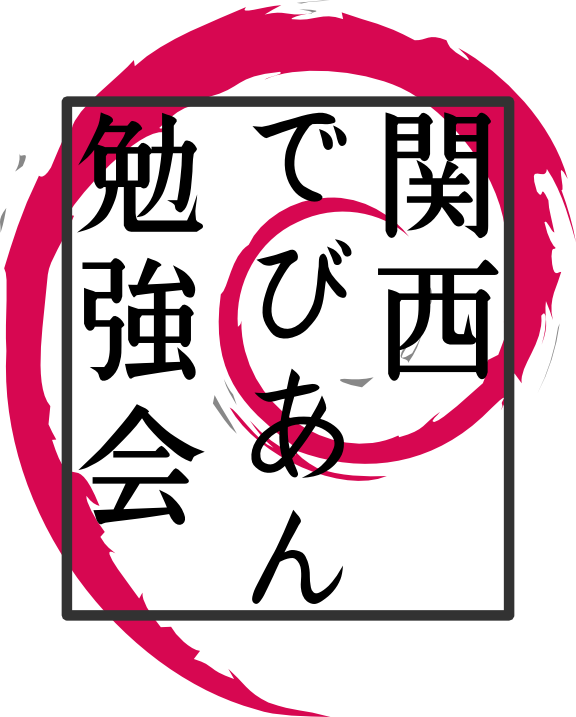
\includegraphics{image200802/kansaidebianlogo.png}
\end{center}

\begin{flushright}
\hfill{}関西 Debian 勉強会担当者 佐々木・倉敷・のがた \\
\hfill{}\debmtgyear{}年\debmtgmonth{}月\debmtgdate{}日
\end{flushright}

\thispagestyle{empty}
\end{titlepage}

\dancersection{Introduction}{Debian JP}

\subsection*{}%ロゴ用のスペース稼ぎ

関西 Debian 勉強会は Debian GNU/Linux のさまざまなトピック (新しいパッケー
ジ, Debian 特有の機能の仕組, Debian 界隈で起こった出来事, などなど) に
ついて話し合う会です.

目的として次の三つを考えています.
\begin{itemize}
      \item ML や掲示板ではなく, 直接顔を合わせる事での情報交換の促進
      \item 定期的に集まれる場所
      \item 資料の作成
\end{itemize}

それでは, 楽しい一時をお楽しみ下さい.

\clearpage

\begin{minipage}[b]{0.2\hsize}
 {\rotatebox{90}{\fontsize{80}{80}
{\gt 関西 Debian 勉強会}}}
\end{minipage}
\begin{minipage}[b]{0.8\hsize}
\hrule
\vspace{2mm}
\hrule
\setcounter{tocdepth}{1}
\tableofcontents
\vspace{2mm}
\hrule
\end{minipage}

\dancersection{最近の Debian 関係のイベント報告}{Debian JP}

\subsection{squeeze いよいよついにリリース……か……?}
この原稿を書いている時点で、
squeeze のリリース日程として、具体的に 2 月 5 日前後という話がでてきています(RC バグもついに残り 39 という状況です)。
期待しすぎるのも危険ですが、次回の勉強会では squeeze を安定版として語りたいですね。
\begin{figure}[h!]
  \centering
  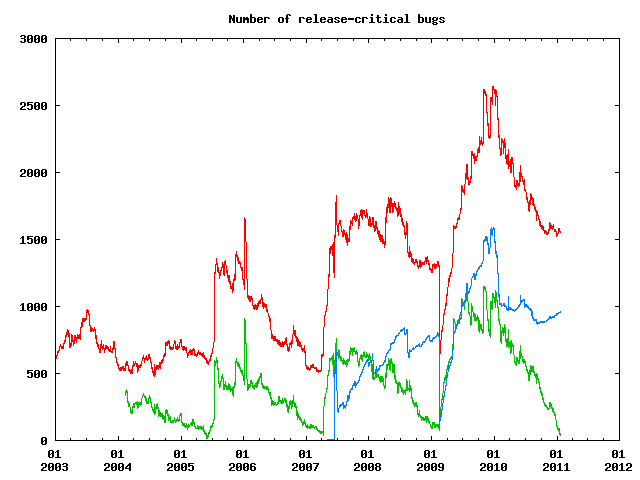
\includegraphics[width=0.7\textwidth]{./image201101/rc-status-20110123.png}
  \caption{現状の RC バグの状況. 緑の線が「次期リリースに関連する RC バグの数」です. 本原稿執筆時点では残り 39 個です.}
\end{figure}

そんな中、2011/01/22 に(日本時間では 23 日未明, つまりこの原稿を書いている時に)
Lenny 最後の point release(になるであろう) 5.0.8 がリリースされました\footnote{\url{http://www.debian.org/News/2011/20110122}}。


\subsection{第 42 回関西 Debian 勉強会}
前回の関西 Debian 勉強会は 12 月 23 日大阪福島区民センターで開かれました.

森山さんによる「Proxmox VE の紹介」セッションと、関西 Debian 勉強会
の 1 年の振りかえりを行ないました。

Proxmox については、便利なのにあまり知られていないということもあり、
知名度向上に一役買ったのではないでしょうか。
実機デモや実際の活用も交えた紹介で、わかりやすいセッションだったと
思います。インストールさえしてしまえば、中身は普通に Debian ですので、
皆さんも是非使ってみてください。

振りかえりの方は、去年の年初にあがっていた目標の状況おさらいや、今年の
ネタをどう進めていくか、などをディスカッションしました。
途中で検討が少し中だるみしてしまったのは残念でしたが、引き続き開催して
いきますのでよろしくお願いします。提案やご希望などはいつでも歓迎です。

\subsection{第 71 回東京エリア Debian 勉強会}
2010 年 12 月 18 日に開催され, libsane と CACert の話題があったそうです。

\subsection{第 72 回東京エリア Debian 勉強会}
2011年1月15日に開催され、Debian 勉強会のアンケートシステム解説と、
話題の kinnect を Debian で使うセッションがありました。

また、前回に引き続き CACert のサイン会も実施されたようです。最近
東京では CACert が流行っているようですね。

\begin{figure}[h!]
  \centering
  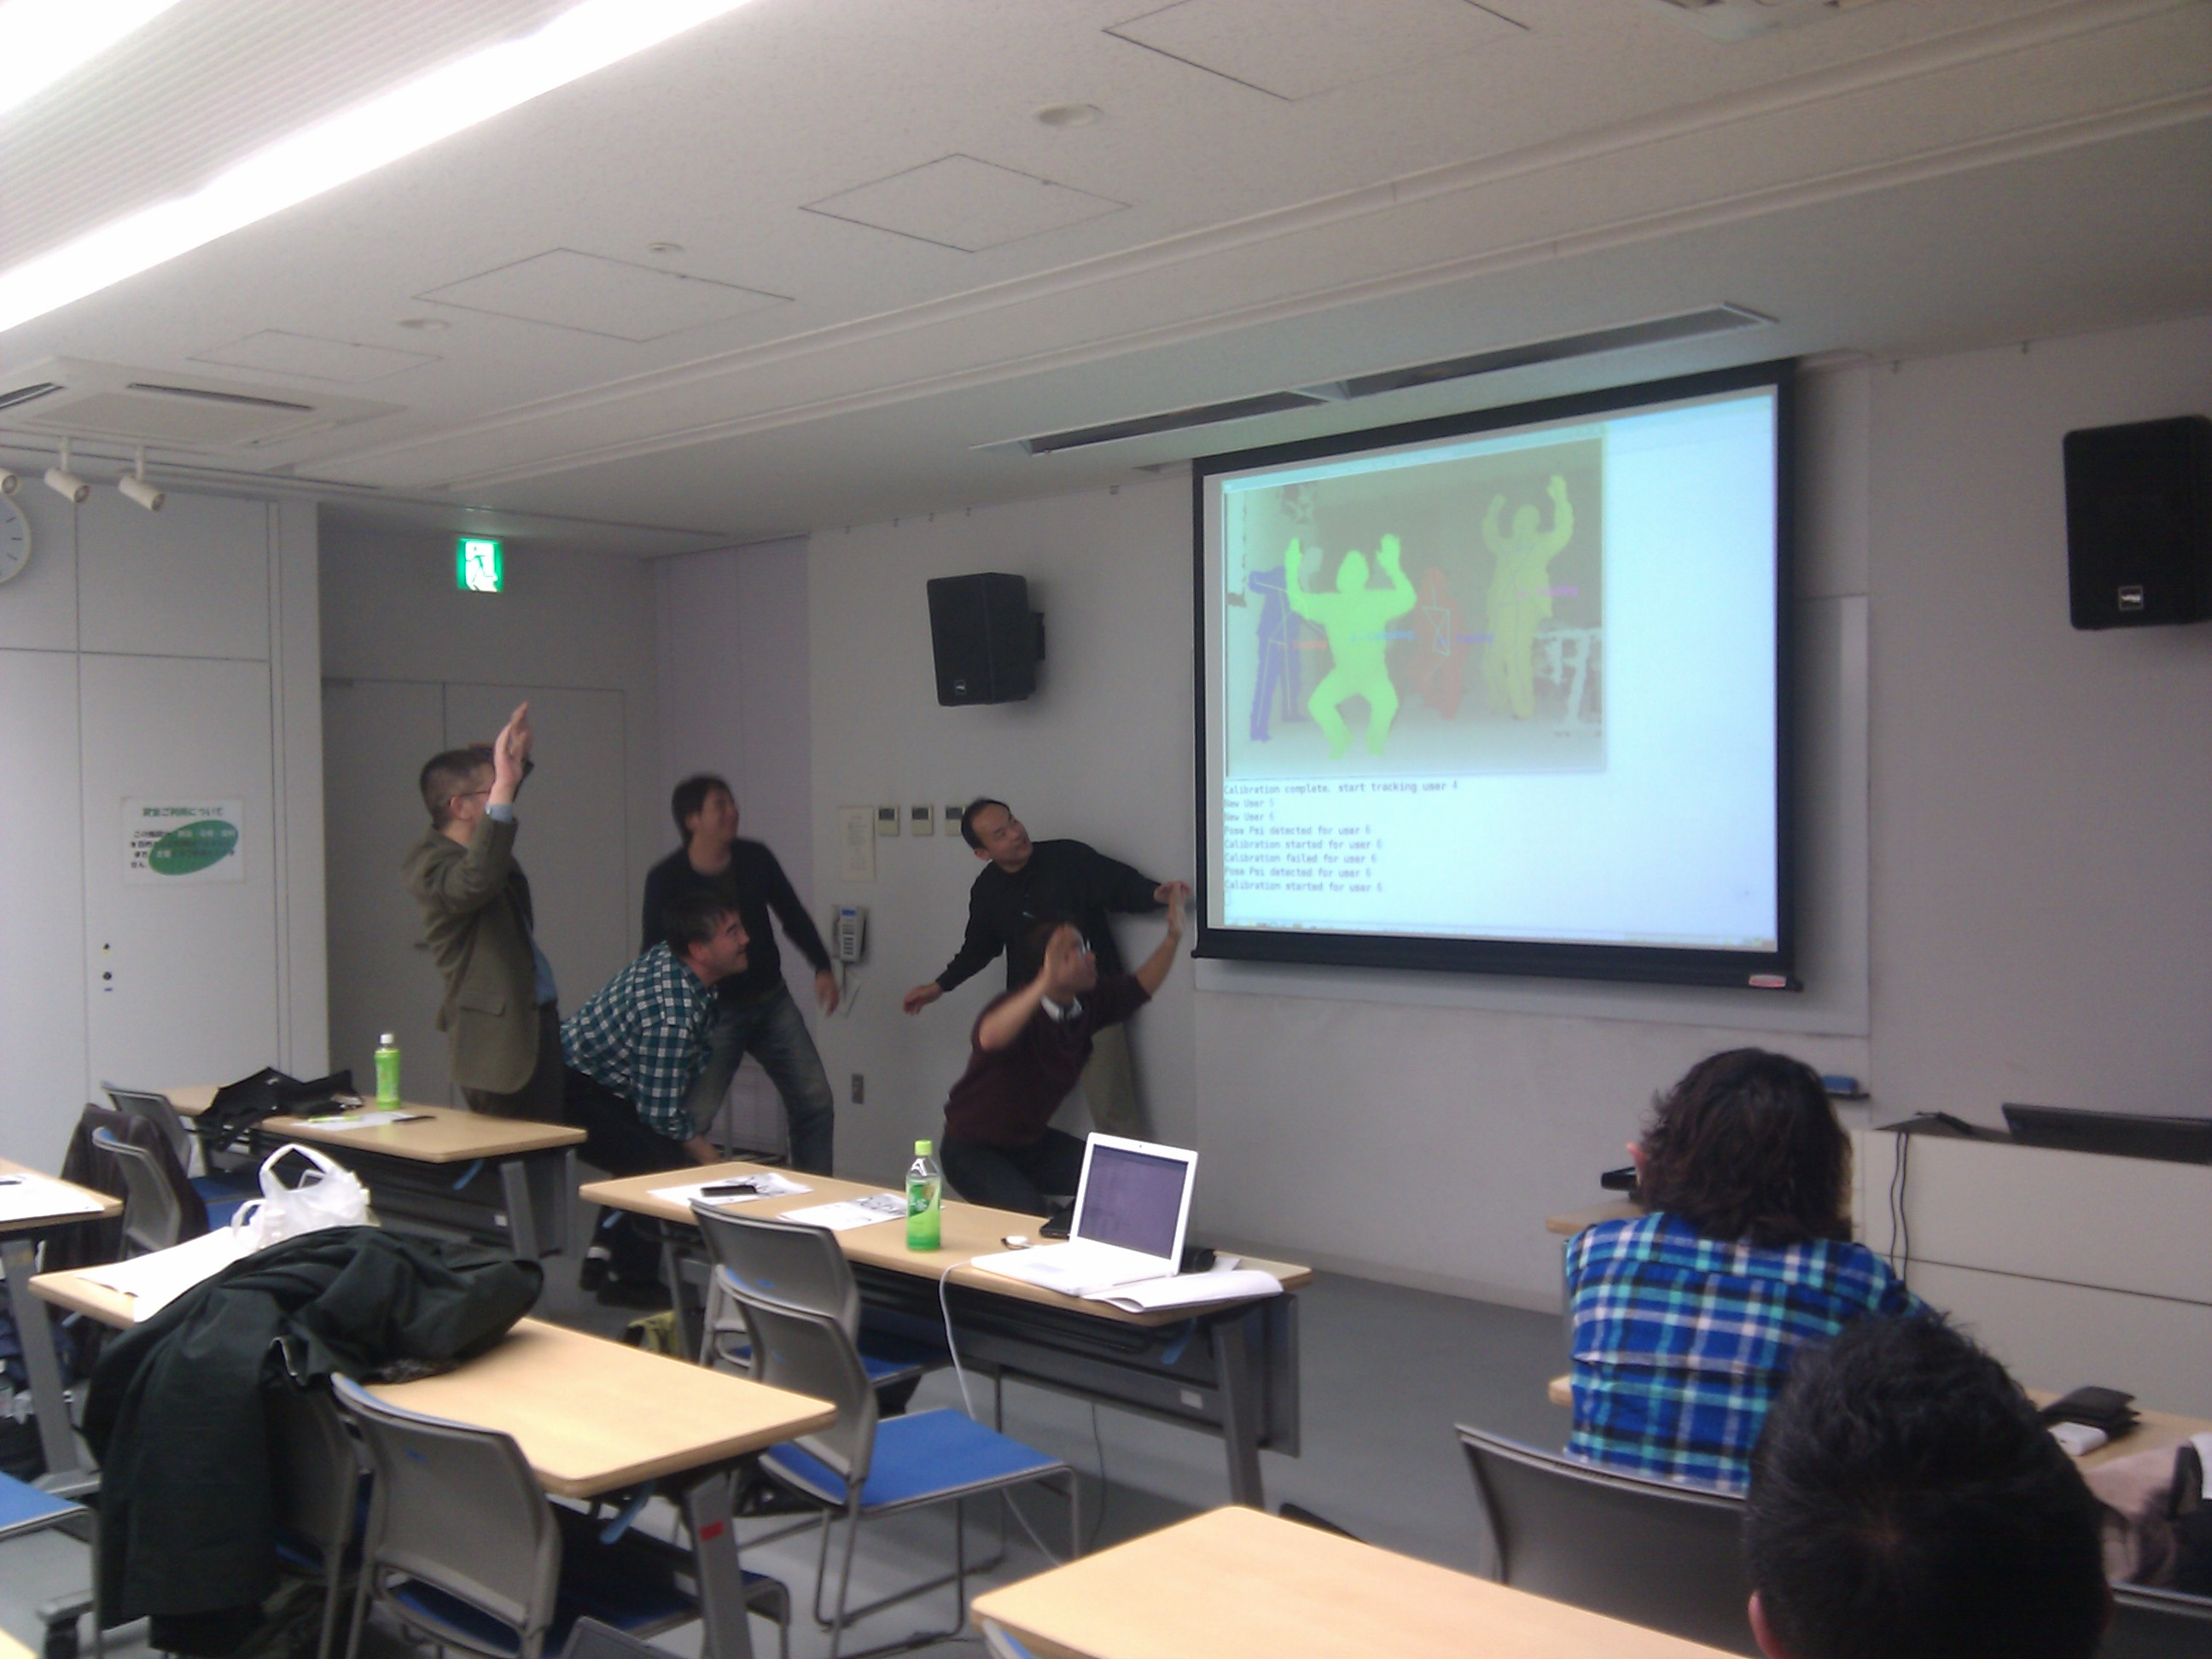
\includegraphics[width=.6\textwidth]{./image201101/kinect.jpg}
  \caption{Kinect で踊る皆さん}
  \label{fig:kinect}
\end{figure}

\clearpage
\dancersection{事前課題}{Debian JP}

今回は以下の課題を設定しました.
%
\begin{quote}
    \begin{screen}
一つバグをみつけてきて下さい. ご意見要望でもかまいません.
    \end{screen}
\end{quote}
%
参加者の皆さんによる回答は以下の通りです.

\begin{prework}{ 甲斐正三 }
  \begin{description}
  \item [未解決事項(私にとって)]
    texworksにおいて日本語が使用できない。
  \item [環境:]
    Debian squeeze,texworks ver0.2.3
  \item [補足:]
    バグなのか、設定が適正でないからなのかわかっていません。
  \item [今後の予定:]
    他のdistroでも同様なのか確認してみます。
  \item [Texの用途:]
    タイミングチャート(図)を含む文章を整形したい。
  \item [その他:]
    申込が遅くなり申し訳ございません\footnote{いえいえ. 毎度ご参加ありがとうございます(佐々木)}。
  \end{description}
\end{prework}

\begin{prework}{ かわだてつたろう }

当日までに何かみつけます。。。

\end{prework}

\begin{prework}{ 山田 洋平 }

去年、はじめてバグを報告し、パッケージを修正してもらえました。
今回は要望を挙げてみたいと思います。日本語環境を改善したいので、当日までに状況を調べて来ます。

\end{prework}

\begin{prework}{ 八津尾 }

要望: Anthyの学習量上限を増やして欲しいなぁ

\end{prework}

\begin{prework}{ dictoss(杉本 典充) }

kfreebsd-amd64環境で、iceweaselで使っているときにハイパーリンク部のテキストをクリックするとフリーズする場合がある。このとき、タブの読み込み中のくるくる回るアニメーションもフリーズする。
\end{prework}



\begin{prework}{ 佐々木洋平 }
  \begin{itemize}
  \item yaskkserv: daemon が動作していない時に /etc/init.d/yaskkserv restart すると error
    \begin{commandline}
      % sudo /etc/init.d/yaskkserv stop
      % sudo /etc/init.d/yaskkserv restart
      Restarting yaskkserv: yaskkservkill: 297: Usage: kill [-s sigspec | -signum | -sigspec] [pid | job]... or
      kill -l [exitstatus]
    \end{commandline}
  \item howm: howm-vars.el を byte-compile すると old-style backqoutes\footnote{原稿執筆時に修正箇所に気がついたので直してしまいましたが...}
  \item elscreen: emasc22 は elscreen 使うと, 起動時にファイルが開けません.
    \begin{itemize}
    \item unstable ではなおってますので backports しましょう.
    \end{itemize}
  \item ptex-base,ptex-bin (wishlist): UTF-8 が通りません.
  \end{itemize}
\end{prework}

\begin{prework}{ dpqpqb }

lenny のシャットダウン中にハングする場合が有る.
仕方無しに電源ボタンの長押しで対処してます.
\begin{itemize}
\item Debian 5.0.8
\item Kernel 2.6.26-2-686
\item GNOME  2.22.3
\end{itemize}
\end{prework}

\begin{prework}{ 山下康成 }

http://www.debian.org/releases/squeeze/armel/apds03.html.ja
D.3.4.1. デバイスファイルの作成 には,
\begin{commandline}
次のようにして, デフォルトの静的デバイスファイル群を作成します.

# cd /dev
# MAKEDEV generic
\end{commandline}
との記述がありますが, 記述の通りに実行すると,
\begin{commandline}
# MAKEDEV generic
.udevdb or .udev presence implies active udev.  Aborting MAKEDEV invocation.
#
\end{commandline}
となります
\end{prework}

\begin{prework}{ 川江 }

バグについてですが, 以前にも話した事があるようにスクリプトやパッケージが自分の「意図」と異なる動きをしたときに, それが「バグ」なのか「設定ミス」なのか分からないときがあります. Xen で言えば時刻の設定や iptables で forward を有効に設定した場合に各 DomainU が外部に接続できなくなるなどです.
\end{prework}

\begin{prework}{ 松澤二郎 }

reportbug がローカライズされていない. gettext のラッピングさえしてなさげ.
(むしろ意図的? 当然英語を使えよな, と暗にほのめかしている気もする)
\end{prework}

\begin{prework}{ bpasao }

(無回答)

\end{prework}

\begin{prework}{ lurdan }

{\url{http://bugs.debian.org/cgi-bin/bugreport.cgi?bug=607721}}

ITP のサンプルです.
\end{prework}

\begin{prework}{ のがたじゅん }

gpsbabel-gui パッケージで desktop ファイルがないのでメニューに反映されない.

\end{prework}

\dancersection{Debian GNU/kFreeBSD で便利に暮らすための Tips}{杉本典充}

\subsection{Debian GNU/kFreeBSD について}
Debian GNU/kFreeBSD とは, Debian Project で開発しているオペレーティングシステムのひとつです. Squeeze にて技術プレビュー版としてリリースされることになっています. \footnote{http://www.debian.org/ports/kfreebsd-gnu/}

\subsubsection{Debian GNU/kFreeBSD の現状}
Debian GNU/kFreeBSD は現在次のような状況です.

\begin{itemize}
  \item カーネルは FreeBSD 8.1 ベースのものに一本化された. (7.3 カーネルは廃止).
  \item まだ Linux バイナリ互換機能は動かない模様. (linux.ko のロード自体に失敗する).
  \item FreeBSD 本家では 8.2 のリリースが間近のため, Debian GNU/kFreeBSD でもアップデートを作業中 (2011/1/12 にカーネルの新しいバージョン 8.2-rc1 がアップロードされた).
\end{itemize}

\subsection{ZFS 環境下でリアルタイム系アプリケーションを使用する Tips}
\subsubsection{現象}
私の PC 環境では, sftp を実行してサーバから 1GB のファイルをダウンロードすると, audacious で再生中の MP3 ファイルが音飛びします. ディスクのアクセス LED は「消灯, 数秒間連続点灯, 消灯」を繰り返すようなディスクアクセスをしており, 音飛びは HDD LED が点灯中に発生します.

なお, PC の環境は以下です.

\begin{itemize}
  \item ノート PC の VAIO TZ. 2.5inch HDD (SATA150 接続) の 250GB.
  \item / は UFS, /home は ZFS としている.
  \item ZFS の設定で, 圧縮はしない (compression=off) 設定にしている.
  \item 再生する MP3 ファイルと sftp でダウンロードする 1GB のファイルは双方 ZFS 領域に読み書きする.
\end{itemize}

\subsubsection{原因の推定}
ディスクのアクセス LED が点灯しているときに MP3 ファイルの再生が音飛びするため, 1GB のファイルを書き込み中に MP3 ファイルの読み込みが行えななかったためと推測します.

そのため, 大きいファイルを書き込む場合でもディスクへの連続書き込み時間を短くするように ZFS のパラメータを調整すれば現象は解決すると考えます.

ZFS のパラメータ設定については FreeBSD を使う人たちで研究されており, その結果が公開されています. \footnote{http://wiki.freebsd.org/ZFSTuningGuide}

\subsubsection{ZFS のパラメータを調整する}
ZFS のパラメータを表示するには"sysctl''コマンドを使用します.
今回調整するパラメータは'vfs.zfs.arc\_max'のため, 現在の値を確認します.

\begin{commandline}
$ sysctl -a | grep arc_max
vfs.zfs.arc_max: 428705280
\end{commandline}

デフォルト値は約 400MB に設定されています.

FreeBSD における ZFS のパラメータ設定は"/boot/loader.conf''に記述するのですが, Debian GNU/kFeeeBSD では"/boot/loader.conf''に記述しても効きません.
また, カーネルの起動後に"sysctl'コマンドを直接実行してもすでに ZFS subsystem が起動しているため変更できない状況です.

そのため, grub の起動パラメータとして設定する方法をとりました.

\begin{commandline}
$ sudo vim /etc/grub.d/10_kfreebsd
# (省略)
# 元から設定しているパラメータ
set kFreeBSD.vfs.root.mountfrom=${kfreebsd_fs}:${kfreebsd_device}
set kFreeBSD.vfs.root.mountfrom.options=rw

# 今回新しい設定値を追加します.
set kFreeBSD.vfs.zfs.arc_max="100M"
# (省略)
$ sudo update-grub
$ sudo reboot
\end{commandline}

\subsubsection{確認}

\begin{commandline}
$ sysctl -a | grep arc_max
vfs.zfs.arc_max: 104857600
\end{commandline}

設定した通り, 100MB になりました.
これでテストしてみると音飛びがしなくなりました.

このパラメータ値はハードウェア環境, ディスク負荷で個々に違ってくるため, 皆さんの使い方に合わせてチューニングしてみてください.

\subsection{USB メモリのマウントに関する Tips}
\subsubsection{まず普通にやってみる}
私の Debian GNU/kFreeBSD 環境は"ja\_JP.UTF-8''の locale を使用しています.
FAT32 でフォーマットしている USB メモリに日本語ファイル名をもつファイルがある場合は mount 時に文字コードの変換が必要になります.
そのため, 文字コード変換のオプションを指定してマウントを試みます.

すると"libiconv.so''がないといわれ, エラーになります.

\begin{commandline}
$ sudo mount_msdosfs -L ja_JP.UTF-8 -D CP932 /dev/da0 /mnt/usb
mount_msdosfs: Unable to load iconv library: libiconv.so: cannot open shared object file: No such file or directory
: No such file or directory
mount_msdosfs: msdosfs_iconv: No such file or directory
\end{commandline}

\subsubsection{libiconv のビルド}
しかし Debian には libiconv.so というライブラリファイルは存在しません.
そのため, GNU のサイトから tarball をダウンロードして build することにします.

\begin{commandline}
$ cd
$ mkdir tmp
$ wget http://ftp.gnu.org/pub/gnu/libiconv/libiconv-1.13.1.tar.gz
$ tar zxvf libiconv-1.13.1.tar.gz
$ cd libiconv-1.13.1
$ ./configure
$ make
$ sudo make install
$ ls /usr/local/lib
charset.alias  libcharset.so        libiconv.la    libiconv.so.2.5.0
libcharset.a   libcharset.so.1      libiconv.so    python2.6
libcharset.la  libcharset.so.1.0.0  libiconv.so.2  site_ruby
\end{commandline}


再度 mount を試みます.
コマンド自体はエラーになりませんが, /mnt/usb の中を ls してみると, 日本語部分が
? で表示されています. 文字コードの変換に失敗したようです.

\begin{commandline}
$ sudo mount_msdosfs -L ja_JP.UTF-8 -D CP932 /dev/da0 /mnt/usb
\end{commandline}

\subsubsection{文字コード変換の失敗原因}
FreeBSD 本家のカーネルでも mount\_msdosfs で UTF-8 へ文字コードを変換する処理は動作しないようです. \footnote{日本語の UTF-8 へファイル名を変換して mount できるようにするパッチは FreeBSD を使う有志によって作成されているようですが, GENERIC カーネルに取り込まれていないようです. }
そのため, 考えられる方法は以下の 3 つありそうです.

\begin{itemize}
  \item USBメモリに日本語ファイル名を使わない。(他人からもらったデータの場合は都合が悪い場合もある。)
  \item localeの設定を''ja\_JP.eucJP'で運用する。(eucJPへの変換は動作するため)
  \item 一時的にlocaleを''ja\_JP.eucJP''に設定してUSBメモリからHDDにコピーし、convmvでUTF-8へファイル名を変換する。その後、localeを''ja\_JP.UTF-8''に戻す。
\end{itemize}

私の環境ではすでに UTF-8 の文字コード環境を使っている都合上, convmv を使った方法を紹介します.


まずは, ja\_JP.eucJP 環境で起動します.
\begin{commandline}
$ vim .xinitrc
# export LANGUAGE='ja_JP.UTF-8'
# export LC_ALL='ja_JP.UTF-8'
# export LANG='ja_JP.UTF-8'
export LANGUAGE='ja_JP.eucJP'
export LC_ALL='ja_JP.eucJP'
export LANG='ja_JP.eucJP'
$ startx
\end{commandline}

ファイルを一度 HDD にコピーし, コピーしたファイル名の文字コードを変換します.
\begin{commandline}
$ sudo mount_msdosfs -L ja_JP.eucJP -D CP932 /dev/da0 /mnt/usb
$ mkdir ~/usbtmp
$ cd ~/usbtmp
$ cp -r /mnt/usb/* ./
$ convmv -r -f eucjp -t utf8 * --notest
\end{commandline}

locale を元に戻します.

\begin{commandline}
$ vim .xinitrc
export LANGUAGE='ja_JP.UTF-8'
xxport LC_ALL='ja_JP.UTF-8'
export LANG='ja_JP.UTF-8'
# export LANGUAGE='ja_JP.eucJP'
# export LC_ALL='ja_JP.eucJP'
# export LANG='ja_JP.eucJP'
$ startx
\end{commandline}

一手間必要ですが, locale を"ja\_JP.UTF-8"で使う場合はこのような回避策を行うことで対応することができます.

\subsection{今後の課題}
日常生活で使えると便利な以下の事項については, 現在調査中です.

\begin{itemize}
  \item iceweasel がよくフリーズする. (代わりに epiphany-browser を使用している).
  \item Flash はやはり鬼門で安定して動作できていない. (gnash はひとまず purge している).
  \item VAIO TZ の液晶の明るさ変更 (Fn キーから音量は何もしなくても変更できているが…).
  \item 無線 LAN (iwn0 として内蔵無線 LAN カードの認識はできているがエラーになる)
  \item IS03 を使ってテザリングする. (まずはドライバをなんとかしないと)
\end{itemize}

\subsection{終わりに}
Debian GNU/kFreeBSD はこれから更に完成度を高めていけるオペレーティングシステムのため, オペレーティングシステムの開発に関わりたい人には打ってつけのプロジェクトです.
今後も Debian GNU/kFreeBSD を使い, デバッグしながらいろいろ勉強していきたいです.

%-------------------------------------------------------------------------------

\dancersection{バグ報告はバグのためだけじゃないよ}{のがたじゅん}

%-------------------------------------------------------------------------------

\subsection{はじめに}

Debianを使っている時、なにか不具合を見つけたとします。
そんな時、あなたはどういう行動をとるでしょうか。

Sidを使っていてよくあるケースは、パッケージのアップデート直後に以前と違う
動きをしてバグに気がつくというケースでしょう。

そんな時、/var/log/apt/term.logや/var/log/aptitudeのログを見て、アップデー
トしたパッケージにアタリをつけ、Debianバグ管理システム(BTS:Bug Tracking
System)\footnote{\url{http://bugs.debian.org/}}にそのパッケージのバグ情報
を見に行きます。

すると、あなたの遭遇したバグはすでに報告されていて、結局何もすることなかっ
た。で終わる人も多いかと思います。

そんなあなたのために、今回は不具合報告以外に焦点を当てたバグ報告について
書いてみたいと思います。

\subsection{おさらいも兼ねてバグ報告の基本}

バグ報告以外のBTSの使い方、といっても基本的なバグ報告について知らなければ
応用もできないので、おさらいも兼ねてバグ報告の基本について述べます。

DebianのBTSは、debbugsと呼ばれるDebianに特化したバグ報告システムを使って
います。
debbugsはメールベースのBTSで、submit@bugs.debian.org宛にメールを送ること
でバグを登録できます。

メールの送り方は、メールのSubjectにバグの内容についての要約を書きます。メー
ル本文にはBTSとして受け付けてもらうための擬似ヘッダを書きます。書き方は本
文1行目にパッケージ名、2行目にパッケージのバージョンを書きます。
必要に応じて重要度とタグを書き、その後にバグの内容を書いていきます。

\begin{commandline}
Subject: バグについて
----
Package: <パッケージ名>
Version: <パッケージバージョン>
Severity: <重要度 critical|grave|serious|important|normal|minor|wishlist>
Tags: <タグ>

以下バグの内容を書く
\end{commandline}

\subsubsection{reportbug/reportbug-ng/debian-elを使う}
Debianのバグ報告の基本は以上ですが、バグ報告のたびに毎回手で書くのは非常
に面倒です。

reportbugやreportbu-ngを使うと定型化された部分は自動で埋めて、バグ修正に
必要な情報も付記してくれるので、バグ報告にはこれらを利用しましょう。

reportbugを初めて使う場合はターミナルからはreportbug、GUIからは[メ
ニュー]→[システムツール]→[reportbug]を実行すると、reportbugの初期設定が
始まります。

詳しい初期設定の方法については「あんどきゅめんてっどでびあん2009年冬号」
の「GUIがついて格好良くなったreportbugを使ってみよう」\cite{nogata2009}に
書いてあるので参考にしてください。

reportbug-ngを使う場合は、普段使うメーラー(MUA)と連携して利用するので、
reportbug-ngのメニューバー[Edit]のMail ClientでMUAを確認しておきます。

emacsの人はdebian-elパッケージを入れておいて、M-x debian-bugでいいと思い
ます。

\subsubsection{reportbugを使ったバグ報告の仕方}

reportbugを使ってバグを報告するには、reportbugをそのまま起動するとバグ報
告をしたいパッケージ名を尋ねられるので入力するか、reportbugにパッケージ名
をつけて起動します。

\begin{commandline}
 $ reportbug (パッケージ名)
\end{commandline}

パッケージ名を入力すると、そのパッケージの既存のバグ一覧が表示されるので、
目を通して、同じものがなければバグ報告に進みます。

reportbugの一連の流れも「あんどきゅめんてっどでびあん2009年冬号」の「GUI
がついて格好良くなったreportbugを使ってみよう」\cite{nogata2009}に書いて
あるので参考にしてください。

\subsection{Severity(バグの重要度)とTags(タグ)}
バグ報告の基本で擬似ヘッダに書くSeverity(バグの重要度)とTags(タグ)につい
て触れましたが、ここでは「Debian -- Debian BTS ― 開発者情報」
\footnote{\url{http://www.debian.org/Bugs/Developer}}から引用して、簡単に
説明します。

\subsubsection{Severity(バグの重要度)}
バグの重要度はcritical(致命的)から、wishlist(要望)までの7段階に分かれて
います。通常使うのはnormalが多いと思います。


\begin{description}
 \item[critical (致命的)]

            システム上の関係のないソフトウェア (またはシステム全体) を破
            壊する、重大なデータの欠落を引き起こす、または、そのパッケー
            ジをインストールしたシステム上でセキュリティホールが生じる場
            合。

 \item[grave (重大)]

            問題のあるパッケージが使用できない、またはほ
            とんど使用できない。またはデータの欠落を引き起こす、そのパッ
            ケージを使用するユーザのアカウントにアクセスを許してしまうセ
            キュリティホールが生じる場合。

 \item[serious (深刻)]

            Debian ポリシーに対して見すごせない違反がある (大まかに言うと、
            「must」や「required」の要件に違反している)、またはパッケージメ
            ンテナあるいはリリースマネージャの意見としてそのパッケージが
            リリースに適していないと判断された場合。

 \item[important (重要)]

            バグがパッケージの有用性を大きく損なっている場合 (ただし、誰
            にとっても完全に使用できなくなっている場合を除く)。

 \item[normal (通常)]
            デフォルト値。通常のバグ。

 \item[minor (軽度)]

            問題がパッケージの利用に影響しない、かつ修正はたいした事がな
            いと思われる場合。

 \item[wishlist (要望)]

            将来的な要望、主に設計上の理由により修正が非常に困難なバグ。
\end{description}


\subsubsection{Tags(バグのタグ)}
バグ報告には決められたタグをつけることができます。

とりあえず抜き書きをしてみましたが、個人的にはパッチをつけたときにpatchを
使ったことがあるような気がしますが、そんなに意識して使ったことがないです。


\begin{description}
 \item[patch (パッチ)]

            バグ報告に、バグを修正するためのパッチや簡単な手順が含まれて
            います。パッチがあってもバグを適切に解決できない場合や別の問
            題を生じる場合は、 このタグは使うべきではありません。

 \item[security (セキュリティ)]

            このバグはパッケージのセキュリティ問題を説明します (例: アク
            セスされてはいけないデータへのアクセスを許可する不正な許可属
            性がある、 やれるべきではない方法でシステムを制御できるバッ
            ファオーバーフローがある、 修正すべき DoS 攻撃の穴がある、
            等)。ほとんどのセキュリティバグは、critical (致命的) や
            grave (重大) の severity (重要度) も設定すべきです。

 \item[upstream (上流)]

            このバグは、パッケージの上流の部分に影響します。

 \item[l10n]

            このバグは、パッケージの地域化に関するものです。

 \item[sid/squeeze/lenny]

            ディストリビューションに関するタグです。
\end{description}


\subsection{不具合報告ではないバグ報告とは}

バグ報告についてひと通り書きましたが、タイトルにもあるようにDebianはパッ
ケージに由来する不具合のほかに、Debianに関連する問題があれば、すべてBTSに
登録し管理します。

話だけではわかりにくいですが、reportbugを起動してパッケージ名の代わりに
「other」と入力すると、このように登録するカテゴリ一覧が表示されます。

\begin{commandline}
 1 base                  General bugs in the base system
 2 bugs.debian.org       The bug tracking system, @bugs.debian.org
 3 buildd.debian.org     Problems and requests related to the Debian Buildds
 4 buildd.emdebian.org   Problems related to building packages for Emdebian
 5 cdimage.debian.org    CD Image issues
 6 cdrom                 Problems with installation from CD-ROMs
 7 debian-i18n           Requests regarding Internationalization (i18n) of the
                         distribution
 8 debian-maintainers    Problems and requests related to Debian Maintainers
 9 debian-policy         Proposed changes in the Debian policy documentation
10 ftp.debian.org        Problems with the FTP site and Package removal
                         requests
11 general               General problems (e.g., that many manpages are mode
                         755)
12 installation-reports  Problems with installing Debian
13 listarchives          Problems with the WWW mailing list archives
14 lists.debian.org      The mailing lists, debian-*@lists.debian.org.
15 mirrors               Problems with Debian archive mirrors.
16 nm.debian.org         New Maintainer process and nm.debian.org website
17 press                 Press release issues
18 project               Problems related to project administration
19 qa.debian.org         Problems related to the quality assurance group
20 release-notes         Problems with the release notes
21 release.debian.org    Requests regarding Debian releases and release team
                         tools
22 security-tracker      The Debian Security Bug Tracker
23 security.debian.org   Problems with the security updates server
24 snapshot.debian.org   Issues with the snapshot.debian.org service
25 spam                  Spam (reassign spam to here so we can complain about
                         it)
26 tech-ctte             Issues to be referred to the technical committee
27 upgrade-reports       Reports of successful and unsucessful upgrades
28 wiki.debian.org       Problems with the Debian wiki
29 wnpp                  Work-Needing and Prospective Packages list
30 www.debian.org        Problems with the WWW site (including other
                         *.debian.org sites)
\end{commandline}

インストーラやプレスリリース、サイトについての問題といった多岐に渡る問題
について扱っていることがわかると思います。

\subsection{wishlistを使う}

もうひとつ。不具合ではないバグ報告としてはwishlist(要望)があります。

wishlist(要望)とは、パッケージに対しての要望がある場合に使用し、たとえば
パッケージのソフトに対して何か機能を追加してもらいたい場合や、アップスト
リームで新しいバージョンのソフトがリリースされたときに、バージョンアップ
をお願いする場合などに使われます。

wishlistの使い方は簡単で、バグの重要度(severity)にwishlistを指定して通常
のバグ報告をするだけです。

\begin{commandline}
$ reportbug gpsbabel-gui (reportbugにパッケージ名をつけて起動します)

Please briefly describe your problem (max. 100 characters allowed; you can
elaborate in a moment). This will be the bug email subject, so write a concise
summary of what is wrong with the package, for example, "fails to send email"
or "does not start with -q option specified" (type Ctrl+c to exit).
> Please include icon and desktop file. (要望の要約を書きます)
\end{commandline}

reportbugにパッケージ名をつけて起動します。起動すると問題の要約を尋ねられ
るので要望の要約を書きます。

\begin{commandline}
Rewriting subject to 'gpsbabel-gui: Please include icon and desktop file.'
Removing release critical severities, since running in 'novice' mode.
How would you rate the severity of this problem or report?

1 important  a bug which has a major effect on the usability of a package,
             without rendering it completely unusable to everyone.

2 normal     a bug that does not undermine the usability of the whole package;
             for example, a problem with a particular option or menu item.

3 minor      things like spelling mistakes and other minor cosmetic errors
             that do not affect the core functionality of the package.

4 wishlist   suggestions and requests for new features.

Please select a severity level: [normal] 4 (wishlistを指定します。)
\end{commandline}

バグの重要度を尋ねられるので、4番のwishlistを選びます。

\begin{commandline}
Spawning sensible-editor... (エディタが起動します)

Subject: gpsbabel-gui: Please include icon and desktop file.
Package: gpsbabel-gui
Version: 1.4.2-1
Severity: wishlist

*** Please type your report below this line ***
(ここに要望の内容を書きます)

(以下略)
\end{commandline}

「*** Please type your report below this line ***」以下に要望を書き終えれ
ば、通常のバグ報告と同じようにsubmit@bugs.debian.orgにメールを送るだけです。

\subsection{パッケージ作成にまつわるバグ報告}

パッケージ作成にまつわるバグ報告と書きましたが、「パッケージがないのにバ
グ報告とははなんぞや?」と思われるかもしれません。

パッケージを作成するためには、「こんなパッケージを作って欲しい」というパッ
ケージ作成希望をバグ報告として出すことからスタートします。

「不具合ではないバグ報告」の章を思い出すと、こういうセクションがあったと
思います。

\begin{commandline}
29 wnpp                  Work-Needing and Prospective Packages list
\end{commandline}

このWNPP(Work-Needing and Prospective Packages)からパッケージ作成が始ま
ります。

(と偉そうに書いていますがWNPPをしたことがないので、Debian -- 作業が望まれ
るパッケージ: \url{http://www.debian.org/devel/wnpp/}に書いてあることをな
ぞっているだけです。何かあればツッコミをお願いします。)

\begin{commandline}
$ reportbug
Please enter the name of the package in which you have found a problem, or
type 'other' to report a more general problem.
> other
\end{commandline}
reportbugを起動して「other」と入力します。

\begin{commandline}
Please enter the name of the package in which you have found a problem, or
choose one of these bug categories:

 1 base                  General bugs in the base system

(中略)

29 wnpp                  Work-Needing and Prospective Packages list
30 www.debian.org        Problems with the WWW site (including other
                         *.debian.org sites)

Enter a package: 29
\end{commandline}
バグのカテゴリーを尋ねられるので29番のWNPPを選びます。

\begin{commandline}
Are you sure you want to file a WNPP report? [y|N|q|?]? y

1 ITP  This is an `Intent To Package'. Please submit a package description
       along with copyright and URL in such a report.
2 O    The package has been `Orphaned'. It needs a new maintainer as soon as
       possible.
3 RFA  This is a `Request for Adoption'. Due to lack of time, resources,
       interest or something similar, the current maintainer is asking for
       someone else to maintain this package. They will maintain it in the
       meantime, but perhaps not in the best possible way. In short: the
       package needs a new maintainer.
4 RFH  This is a `Request For Help'. The current maintainer wants to continue
       to maintain this package, but they needs some help to do this, because
       their time is limited or the package is quite big and needs several
       maintainers.
5 RFP  This is a `Request For Package'. You have found an interesting piece of
       software and would like someone else to maintain it for Debian. Please
       submit a package description along with copyright and URL in such a
       report.

Choose the request type: 5
\end{commandline}
WNPPの中で何をするのか尋ねられます。

\begin{itemize}
 \item ITP: パッケージを作成する (Intent To Package)
 \item O: パッケージを手放す (Orphaned)
 \item RFA: パッケージを引き取って欲しい (Request for Adoption)
 \item RFH: パッケージの維持を手伝って欲しい (Request For Help)
 \item RFP: パッケージをつくって欲しい (Request For Package)
\end{itemize}

なので5のRFPを選びます。

\begin{commandline}
Please enter the proposed package name: sahana-eden
Checking status database...
Please briefly describe this package; this should be an appropriate short
description for the eventual package:
> Disaster management system made from web2py
\end{commandline}
パッケージの簡単な説明を書きます。書き終えるとエディタが起動します。

\begin{commandline}
Spawning sensible-editor...

Subject: RFP: sahana-eden -- Disaster Management System made by web2py
Package: wnpp
Severity: wishlist

*** Please type your report below this line ***

* Package name    : sahana-eden
  Version         : 0.5.3
  Upstream Author : Name <somebody@example.org>
* URL             : https://launchpad.net/sahana-eden
* License         : MIT/X
  Programming Lang: Python
  Description     : Disaster Management System made by web2py

Sahana Eden is an Emergency Development Environment which allows the
rapid deployment of customisable tools to support the 4 phases of the
Emergency Management Cycle as well as Development & Environment
projects. It is an example of an HFOSS project (Humanitarian FOSS)
\end{commandline}
書き終われば保存してエディタを終了します。

\begin{commandline}
Report will be sent to "Debian Bug Tracking System" <submit@bugs.debian.org>
Wrong line:   Upstream Author : Name <somebody@example.org>
ERROR: you have composed an ITP with fields unchanged from the template; this will NOT be submitted. You should
edit all fields so they contain correct values for your ITP (e to edit) [E|q|?]? 
\end{commandline}
適当に書いてると怒られてしまいました。ということでEで戻って書きなおして
保存、submit@bugs.debian.org宛に送ればRFPはおしまいです。

\subsubsection{RFPをITPにする}
この辺りになると自分でも未知の領域ですが、「作業が望まれるパッケージ」に
よると

\begin{quote}
これをパッケージ化することにしたら、このプログラムが パッケージ化の作業中
ことをほかの人に知らせ、さらにあなたがそのバグの 所有者となるために、 バ
グレポートを「RFP」から「ITP」に改称します。それから ソフトウェアをパッケー
ジ化し、アップロードして、そのパッケージが インストールされたらこのバグを
閉じます。
\end{quote}

とのことなので、control@bugs.debian.org宛に「Debian BTS ― 制御サーバ」
\url{http://www.debian.org/Bugs/server-control.ja.html}を参照してコントロー
ルメールを送ればよいのでしょうか。

\begin{commandline}
owner (バグ番号) !
retitle (バグ番号) ITP: sahana-eden -- Disaster Management System made by web2py
thanks
\end{commandline}

調べきれず終わってしまった…。

\subsection{最後に}
不具合報告だけではないバグ報告を書きましたが、いかがでしたでしょうか。
あまり自分も使うことがない事をまとめたので大変でした。


\begin{thebibliography}{99}
 \bibitem[1]{reportbug}
            Debian -- Debian BTS - バグを報告する
            \url{http://debian.org/Bugs/Reporting}
 \bibitem[2]{wnpp}
            Debian -- 作業が望まれるパッケージ
            \url{ http://www.debian.org/devel/wnpp/}
 \bibitem[3]{devref}
            Debian 開発者リファレンス
            「第5章 パッケージの取扱い方」
            \url{http://www.jp.debian.org/doc/manuals/developers-reference/pkgs.html#newpackage}
 \bibitem[4]{iwamatsu2005}
            岩松伸洋
            「ITPの仕方からアップロードまでの流れ」
            (あんどきゅめんてっどでびあん2005年冬号)
            \url{http://tokyodebian.alioth.debian.org/pdf/debianmeetingresume2005-fuyu.pdf}
            pp. 3 -- 7
 \bibitem[5]{yamane2005}
            やまねひでき
            「claim makes Debian better」
            (あんどきゅめんてっどでびあん2005年冬号)
            \url{http://tokyodebian.alioth.debian.org/pdf/debianmeetingresume2005-fuyu.pdf}
            pp. 26 -- 29
 \bibitem[6]{uekawa2005}
            上川純一
            「debbugs internal」
            (あんどきゅめんてっどでびあん2005年冬号)
            \url{http://tokyodebian.alioth.debian.org/pdf/debianmeetingresume2005-fuyu.pdf}
            pp. 31 -- 38
 \bibitem[7]{kinoshita2008}
            木下達也
            「バグレポートから参加するDebianパッケージ開発」
            (あんどきゅめんてっどでびあん2008年夏号)
            \url{http://tokyodebian.alioth.debian.org/pdf/debianmeetingresume2008-natsu.pdf}
            pp. 76 -- 78
 \bibitem[8]{fujisawa2009}
            藤澤徹
            「MC-MPI/GXP公式パッケージへの道」
            (あんどきゅめんてっどでびあん2009年夏号)
            \url{http://tokyodebian.alioth.debian.org/pdf/debianmeetingresume2009-natsu.pdf}
            pp. 77 -- 83
 \bibitem[9]{nogata2009}
            のがたじゅん
            「GUIがついて格好良くなったreportbugを使ってみよう」
            (あんどきゅめんてっどでびあん2009年冬号)
            \url{http://tokyodebian.alioth.debian.org/pdf/debianmeetingresume2009-fuyu.pdf}
            pp. 61 -- 66
\end{thebibliography}


\dancersection{今後の予定}{Debian JP}

\subsection{次回の関西 Debian 勉強会}
次回の関西 Debian 勉強会は 2 月 27 日 (日), 大阪福島区民センターか大阪港区区
民センターのどちらかで行われる予定です.

発表については未定ですので, みなさまの発表をお待ちしております.

\subsection{4 月神戸 IT フェスティバル + オープンソースカンファレンス 2011Kansai@Kobe}

4 月 15 日 (金), 16 日 (土) に JR 神戸駅すぐの神戸市産業振興センターにて, 神戸 IT フェ
スティバル + オープンソースカンファレンス 2011Kansai@Kobe が開催されますがど
うしましょ.


% 冊子にするために, 4 の倍数にする必要がある.
% そのための調整
%\dancersection{メモ}{}
%\mbox{}\newpage

%\printindex
% \cleartooddpage

 \begin{minipage}[b]{0.2\hsize}
  \rotatebox{90}{\fontsize{80}{80} {\gt 関西 Debian 勉強会} }
 \end{minipage}
 \begin{minipage}[b]{0.8\hsize}

 \vspace*{15cm}
 \rule{\hsize}{1mm}
 \vspace{2mm}
 
\includegraphics[width=2cm]{image200502/openlogo-nd.eps}
 \noindent \Large \bf Debian 勉強会資料\\ \\
 \noindent \normalfont \debmtgyear{}年\debmtgmonth{}月\debmtgdate{}日 \hspace{5mm}  初版第 1 刷発行\\
 \noindent \normalfont 関西 Debian 勉強会 (編集・印刷・発行)\\
 \rule{\hsize}{1mm}
 \end{minipage}

\end{document}
